\documentclass{X:/Documents/Coding/Latex/myassignment}
\title{Modelling with ODEs Assignment 4}

\begin{document}

\maketitle
\begin{enumerate}
	\item 

	\begin{enumerate}
		\item The IVP
		\[\odd yx = x -y +1, \quad y(1) = 2\]

		Expressed as an integral equation:


		%not done
		
		\item This is a linear-inhomogeneous ODE. Solution to the homogeneous analogue:
		\begin{align*}
			\odd{y_h}x = -y_h\\
			\implies y_h = ae^{-x}
		\end{align*}
		Using the method of undetermined coefficients, guess 
		\[y = y_h + bx + c\]
		\begin{align*}
			\odd yx = x -y +1\\
			-ae^{-x} + b = x - ae^{-x} - bx - c + 1\\
			b = x - bx - c + 1\\
		\end{align*}
		\begin{align*}
			b = 1\\
			b+c = 1\\
			\implies c=0
		\end{align*}
		Hence
		\[y = ae^{-x} +x\]

		Applying the initial condition $y(1) =2 $ gives
		\begin{align*}
			y(1) = 1 = ae^{-1} + 1\\
			a = e
		\end{align*}
		Hence
		\[y = e^{1-x} + x\]

		%now use matlab to find the taylor series, and compare to (a)
		
		\item %show that the PL theorem works for the IVP and find the largest x interval that guarantees a unique solution
	\end{enumerate}
	\item 
	\[x'''_j = \sum_{i=0}^3 a_i x_{j+1} + \bigo(h^m)\]

	\begin{enumerate}
		\item %calculate the coefficients a_i
		\item %calculate the order m
		\item %check that the coefficients work for a constant function
		For a constant function, $x$: 
		\[x''' = 0\]
		Hence
		\[\sum_{i=0}^3 a_i = 0\]
		%not done
	\end{enumerate}
	\item 
	\[x' = f(t,x),\quad x(0) = 1\]
	With leapfrog method
	\[x_{n+1} = x_{n-1} + 2h f_n\]
	\begin{enumerate}
		\item %given you used the explicit euler method to get x_1, does this affect the global error of the leapfrog method? how?
		\item %write matlab code to solve using the leapfrog method and Euler's method to find x_1
		%calculate the absolute error e(h) against h for t=1
		%plot log(e) vs log(h) and see that this confirms the order of accuracy for the leapfrog method
		\[x' = -x, \quad x(0)=1\]

		\item %given IVPs of the form from b have solutions
		\[x_n = c_+ \xi_+^n + c_- \xi_-^n, \quad n=2,\ldots\]
		Where
		\[\xi_\pm = -h \pm \sqrt{1+h^2}\]
		%and c_\pm are constants. Why does this mean that the leapfrog method is NOT SUITABLE for the long term behaviour of the IVP. Use the code from b to confirm that this is calculating long term solutions of the IVP 
	\end{enumerate}
\end{enumerate}

\clearpage
\section*{Matlab}
\lstinputlisting{ODEsA4.m}


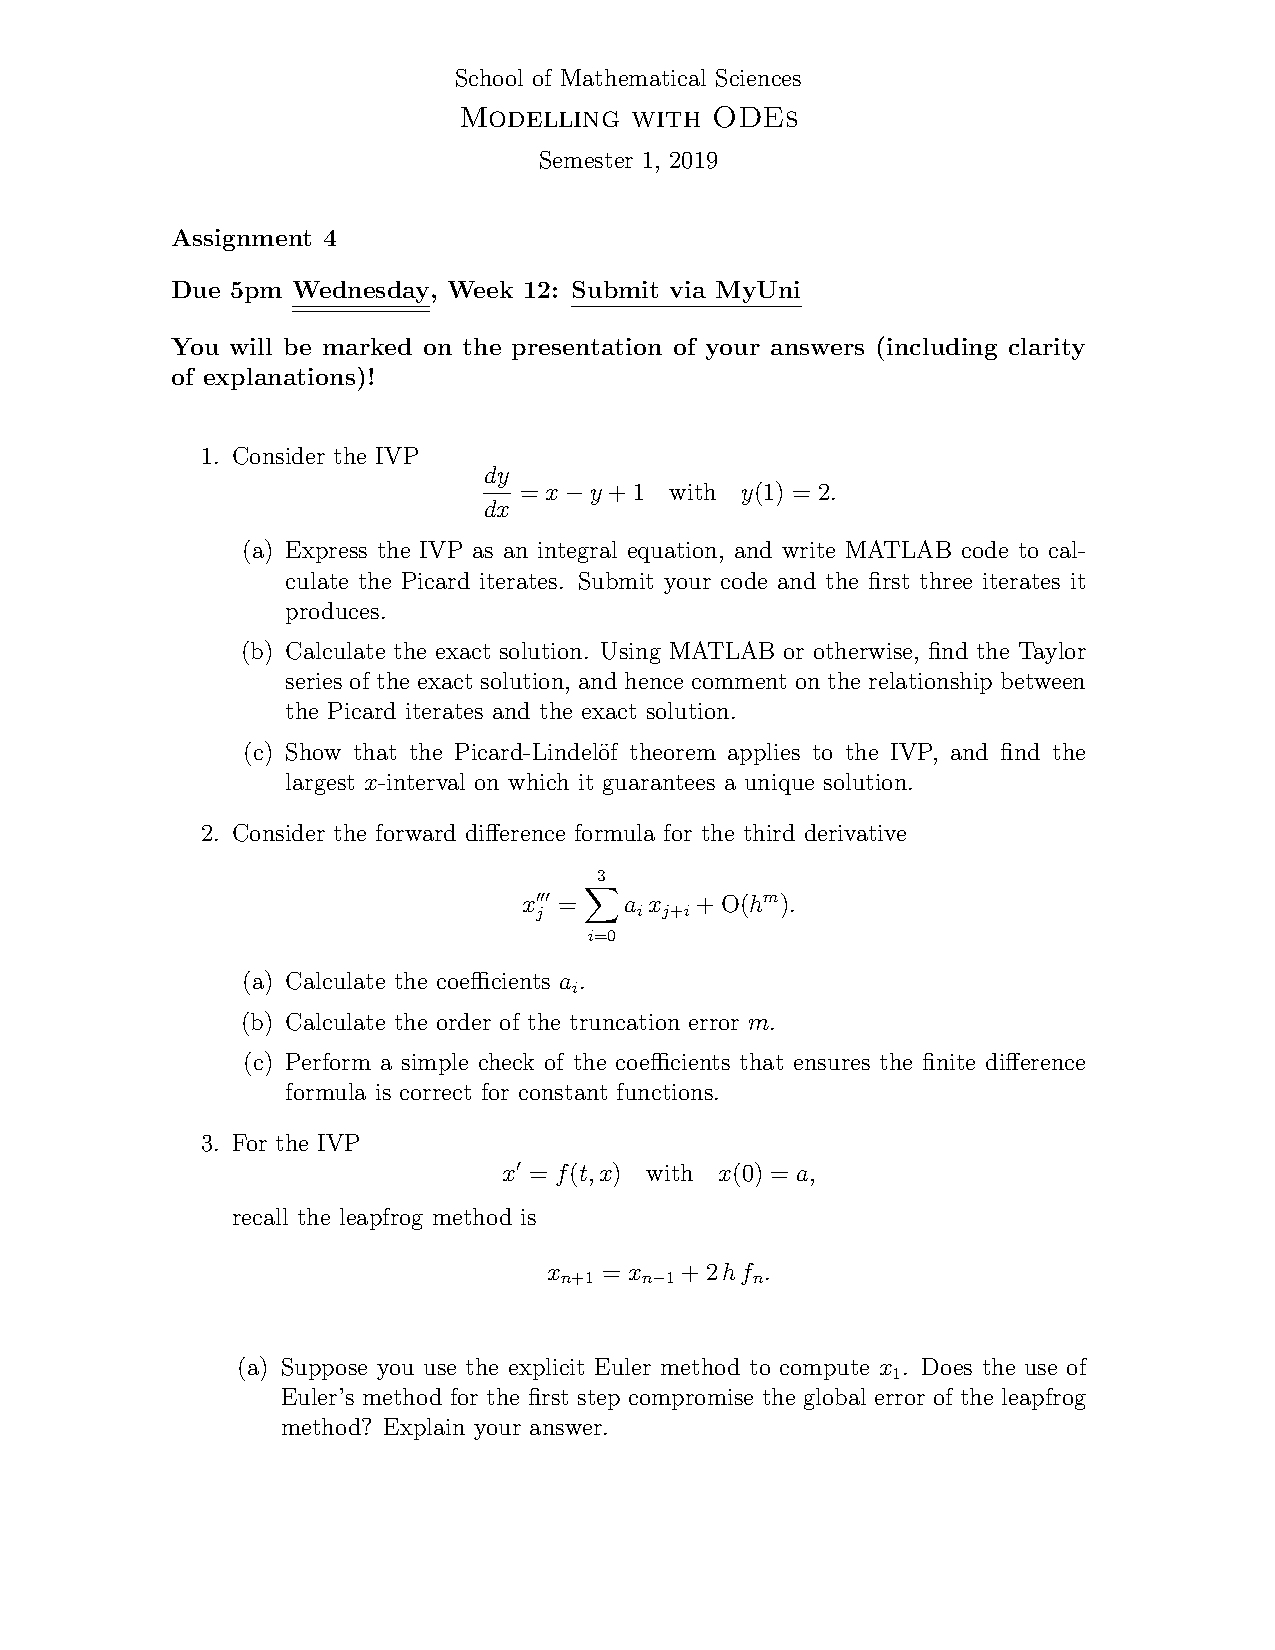
\includepdf[pages=1-]{A4_2019}
\end{document}